\clearpage
\section{Blokkdiagrammer og The Grand Scheme}\label{sec:signal_block_diagram}
I alle fag frem til nå har du sett på et flytdiagram med piler og bokser og tenkt at dette er masse som beveger seg fra en tank til en annen. Ta eksempelet gitt i \cref{fig:simple_blockdiagram}. Hadde vi spurt en kybernetiker hadde han beskrevet figuren som en oversikt over informasjonsflyten til systemet. Som prosessingeniør er det viktig å vite forskjellenene mellom blokkdiagram og flytskjema og deres respektive bruksområder.

\begin{figure}[H]
    \centering
    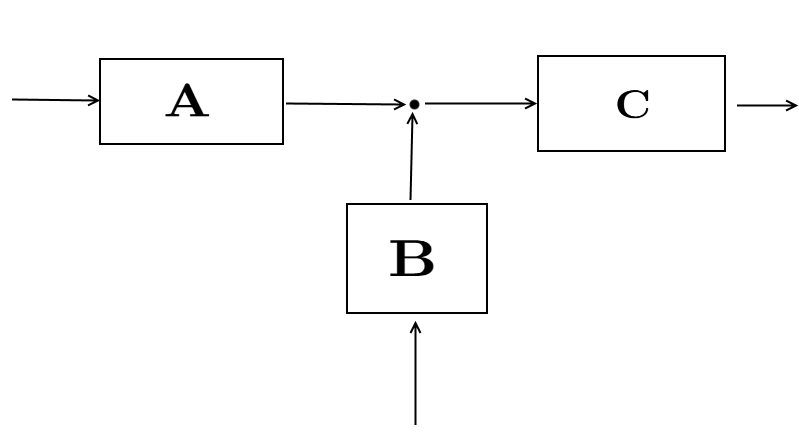
\includegraphics[scale=0.5]{Figures/simple_blockdiagram1.png}
    \caption{Et blokkdiagram.}
    \label{fig:simple_blockdiagram}
\end{figure}

\subsection{Blokkdiagram}
Et blokkdiagram er en visualisering av signaler som sendes fra et system til andre systemer. Til forskjell fra flytskjema er pilene i et blokkdiagram signaler som bærer informasjon istedet for masse. Ved å bruke et blokkdiagram kan vi visualisere hvordan systemer kommuniserer med hverandre i form av lineære sammenhenger.

\begin{figure}[H]
    \centering
    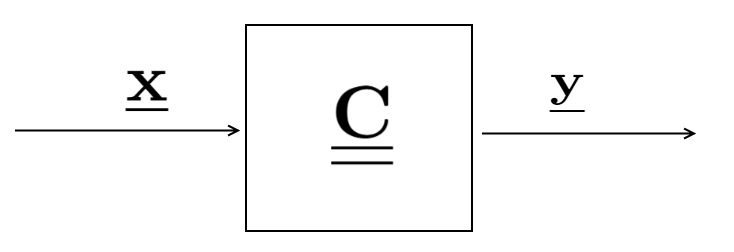
\includegraphics[scale=0.5]{Figures/very_simple_blockdiagram.png}
    \caption{Et veldig enkelt blokkdiagram}
    \label{fig:very_simple_blockdiagram}
\end{figure}

Blokkdiagrammet i \cref{fig:very_simple_blockdiagram} viser den lineære sammenhengen mellom $\underline{\textbf{x}}$ og $\underline{\textbf{y}}$, som kan beskrives som ligningen: 
\begin{equation}
    \label{eq:very_simple_blokkdiagram}
    \underline{\textbf{y}} = \doubleunderline{\textbf{C}}\,\underline{\textbf{x}}
\end{equation}
Trikset med blokkdiagrammer er at alle variablene/vektorene/matrisene ganges med hverandre via en pil og plusses sammen hvis pilen møter en annen pil. Det er mange måter å angripe et blokkdiagram, men en enkel metode er å start bakerst og beveg deg mot pilens retning. Da er du sikker på at du får riktig plassering på vektorer og matriser.

\begin{figure}[H]
    \centering
    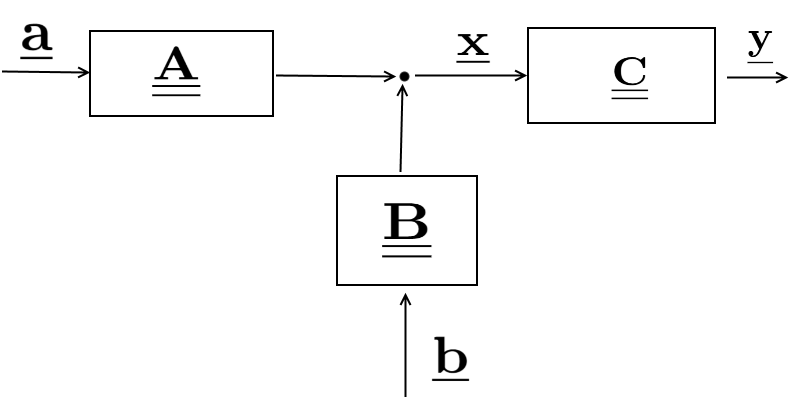
\includegraphics[scale=0.5]{Figures/simple_blockdiagram.png}
    \caption{Blokk diagram med 3 systemer hvor signalet \textbf{y} er en lineær kombinasjon av signalene \textbf{a} og \textbf{b}.}
    \label{fig:simple_blokkdiagram1}
\end{figure}

Fra \cref{fig:simple_blokkdiagram1} er det to ligninger vi kan hente ut. Den første er den samme som i \cref{eq:very_simple_blokkdiagram} og den andre er den lineær kombinasjonen mellom $\doubleunderline{\textbf{A}}\,\underline{\textbf{a}}$ og $\doubleunderline{\textbf{B}}\,\underline{\textbf{b}}$:

\begin{align}
       \label{eq:simple_blokkdiagram}
    \underline{\textbf{y}} =& \doubleunderline{\textbf{C}}\,\underline{\textbf{x}} \\
    \underline{\textbf{x}} =& \doubleunderline{\textbf{A}}\,\underline{\textbf{a}} + \doubleunderline{\textbf{B}}\,\underline{\textbf{b}}
\end{align}

\subsection{The Grand Scheme}
The grand scheme er hele pensum summert opp. Tanken bak The Grand Scheme er at man kan koble sammen alle delene i modellering til et blokkdiagram. I ABC-heftet blir The Grand Scheme forklart ved et blokkdiagrammet gitt i \cref{fig:grand_scheme_hard}:

\begin{figure}[H]
    \centering
    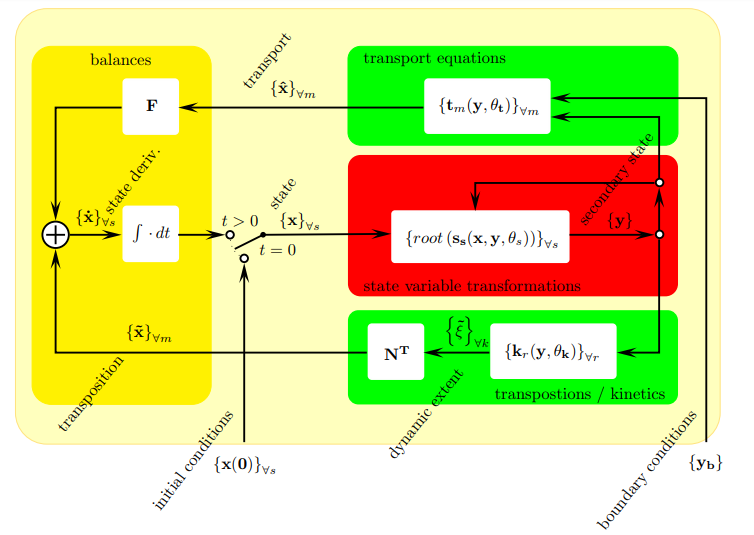
\includegraphics[scale=0.7]{Figures/The_grand_scheme_hard}
    \caption{The Grand Scheme, hentet fra ABC-heftet.}
    \label{fig:grand_scheme_hard}
\end{figure}

Siden dette blokkdiagrammet er litt vanskelig å skjønne har vi laget en versjon som er litt mindre korrekt, men litt mer lesbar når man først introduseres til The Grand Scheme.

\begin{figure}[H]
    \centering
    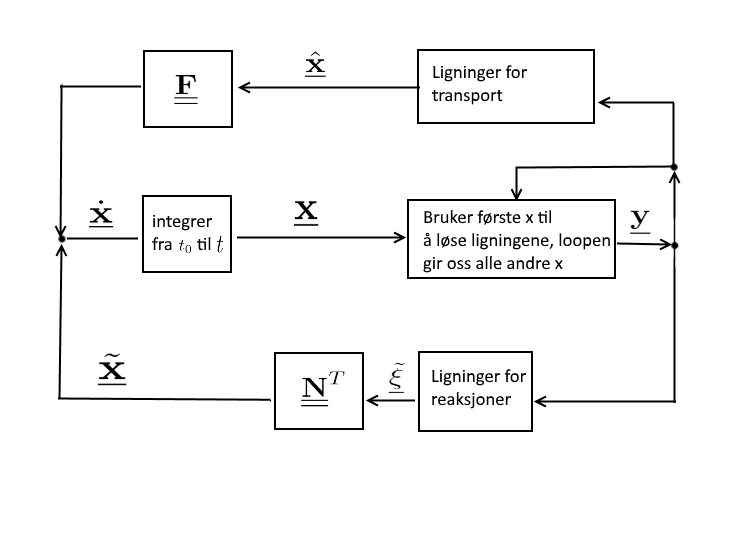
\includegraphics[scale=0.7]{Figures/The_grand_scheme_enkel.png}
    \caption{The Grand Scheme, forenklet.}
    \label{fig:grand_scheme_enkel}
\end{figure}

Bruker vi det vi har lært om blokkdiagrammer og tyder \cref{fig:grand_scheme_hard} i form av linære kombinasjoner får vi et sett med ligninger som beskriver det essensielle i prossmod. Under er $f,g,h$ funksjoner for henholdsvis state, reaksjoner og transport. 

\begin{equation}
\label{eq:The_grand_scheme}
    \begin{split}
    \vecdot{x} =&\, \mymat{F}\,\vechat{x} + \vectil{x} \\
    \vectil{x} =&\, \mymat{N}^T\,\Tilde{\underline{\xi}} \\
    \Tilde{\underline{\xi}} =&\, g(\vec{y}) \\
    \vechat{x} =&\, h(\vec{y}) \\
    \vec{x}_{\text{next state}} &=\, f(\vec{y}) 
    \end{split}
\end{equation}
    
Ligningene over kjenner du forhåpentligvis igjen fra tidligere kapitler. Det er ikke så mye mer å si om The Grand Scheme enn at mesteparten av pensum kan summeres opp i det. 
